\chapter{Implementierung}
% Die grundlegenden Funktionen dieser Arbeit sollen das Erstellen von Veranstaltungen und Benutzern, die Zuweisung untereinander und die Kompatibilität mit mobilen Endgeräten umfassen. Wie diese Funktionen mit Hilfe von modernen Webtechniken implementiert wurden, wird hier beschrieben.

% \section{Problembeschreibung}
% Zur Idee dieser Bachelorarbeit liegt folgende Frage zugrunde:

% \begin{quote}
% 	Kann man eine App entwickeln, in der man zu einer bestimmten Veranstaltung beliebig viele Teilnehmer hinzufügen, deren spezifischen Anmeldedaten hinterlegen und später schließlich verteilt mit beliebig vielen Helfern (mobil) daran arbeiten? 
% \end{quote}

% Diese Fragestellung ist deshalb interessant, weil die App in erster Linie im Oktober am freideutschen Jugendtag verwendet werden soll. Dort werden über 4000 Pfadfinder erwartet, die aus Deutschland, der Schweiz und Österreich stammen und zu verschiedenen Zeiten an- und abreisen werden. Außerdem benötigen einige Gruppen besondere Materialien (vorwiegend verschieden lange Holzstangen für den Bau diverser Zelte), die vorher von den Helfern organisiert werden müssen.

\subsection{Identifizierung des Problems}
Bei dem Gedanken eine App zu entwickeln, steht man oft vor der Entscheidung für welche Plattform man denn entwickeln möchte: Linux, Windows, OS X, iOS, Android, Windows Phone, Blackberry OS etc. Doch das würde voraussetzen, dass alle Benutzer dieser App das gleiche Betriebssystem benutzen. Für eine Veranstaltung, wie das Meißnerlager, eine sehr schlechte Annahme. Die ehrenamtlichen Helfer müssen mit ihren eigenen / privaten Smartphones und Tablets arbeiten. Es ist davon auszugehen, dass es sich dabei um unterschiedliche Geräte mit verschiedenen Betriebssystemen handelt.\par

Wieso also nicht für alle Plattformen gleichermaßen entwickeln? Dank dem Google Projekt \glqq HTML5 Rocks\grqq{}\cite{html5rocksmain} und vielen interessierten Entwicklern ist \emph{HTML5} in aller Munde. Somit gibt es tatsächlich die Möglichkeit, jedes Betriebssystem mit einer einzigen Web-App abzudecken.

\paragraph{Definition Webanwendung} 
Eine Webanwendung, auch \emph{Web-App} genannt, ist eine Anwendung, die vollständig in einem Browser ausführbar ist. Da sie (fast) vollständig auf einem Webserver ausgeführt wird, ist das zugrunde liegende Übertragungsprotokoll \emph{HTTP}.\par

Das Interessante an dieser Art der Anwendung ist, dass sie auch auf Smartphones und Tablets ausgeführt werden können, ohne sie vollständig auf die jeweilige Plattform portieren zu müssen. Das heißt, man entwickelt einmal eine Webanwendung und kann sie dann auf allen gängigen Endgeräten ausführen.\\
Damit wäre ein wichtiges Kriterium für die Nutzung beim Meißner erfüllt: die betriebssystemunabhängige Nutzung.

\paragraph{Auszeichnungssprache HTML5}
\emph{HTML5} ist der angehende Nachfolger des aktuell verwendeten HTML 4.0.1. Es ist immer noch im experimentellen Entwicklungsstand, wird aber durch große Unternehmen wie Google gefördert und erreichte damit auch eine große Beliebtheit. Alle Browser verstehen daher die gängigsten HTML5 Befehle, allerdings werden nie alle Funktionen unterstützt. Der Grundbefehlssatz ist in allen Browsern enthalten, weshalb es schon seit einiger Zeit möglich ist, mit dem neuen angehenden Webstandard seine Webanwendung zu gestalten.

\paragraph{Framework}
Mit der Wahl des Open Source Frameworks \emph{cakePHP} \cite{cakePHP} stehen auch serverseitig \emph{PHP5} und clientseitig \emph{JavaScript} als weitere Sprachen fest. Als Datenbank wird \emph{MySQL} gewählt und für den Webserver kommt \emph{Apache} zum Einsatz, beides ist durch das Entwicklerpaket \emph{XAMPP} gegeben.\par

Außerdem  wurde das Framework \emph{socket.io} \cite{socket.io} gewählt, da es mit wenig Aufwand einen stabilen WebSocket Server bereitstellt. Dieser beinhaltet wichtige Funktionen, wie Broadcast, Fallbacks und Socketverwaltung, welche von dieser Arbeit verwendet werden.

\subsection{Beschreibung der Umgebung}
Da eine Web-App eine Internetverbindung (mindestens zum initialen Laden) benötigt, muss gesichert sein, dass diese auch zur Verfügung steht. Die Webanwendung soll zuerst am Meißnerlager 2013 am Hohen Meißner verwendet werden, wo im Allgemeinen eine schlechte Internetanbindung auf dem Gelände zu erwarten ist, allerdings hat ein großes Telekommunikationsunternehmen die Versorgung zugesichert. Somit ist garantiert, dass die App dort verwendet werden kann.

\section{Struktur der Webanwendung}
Für die Grundstruktur wurde das Open Source Framework cakePHP verwendet. Es verwendet für eine klare Trennung der Logik und dem Design das Entwurfsmuster \emph{Model View Controller}.

\subsection{Entwurfsmuster: Model View Controller}
Befasst man sich mit dem Entwickeln von modernen Webseiten, Apps oder ähnlichen Projekten, so stößt man direkt auf das Muster zur Strukturierung als Model View Controller (\emph{MVC}, deutsch: Modell-Präsentation-Steuerung). Dieses Muster kapselt drei Elemente voneinander und ermöglicht dadurch, dass Änderungen einfach implementiert werden können.

\begin{figure}[!ht]
	\centering
	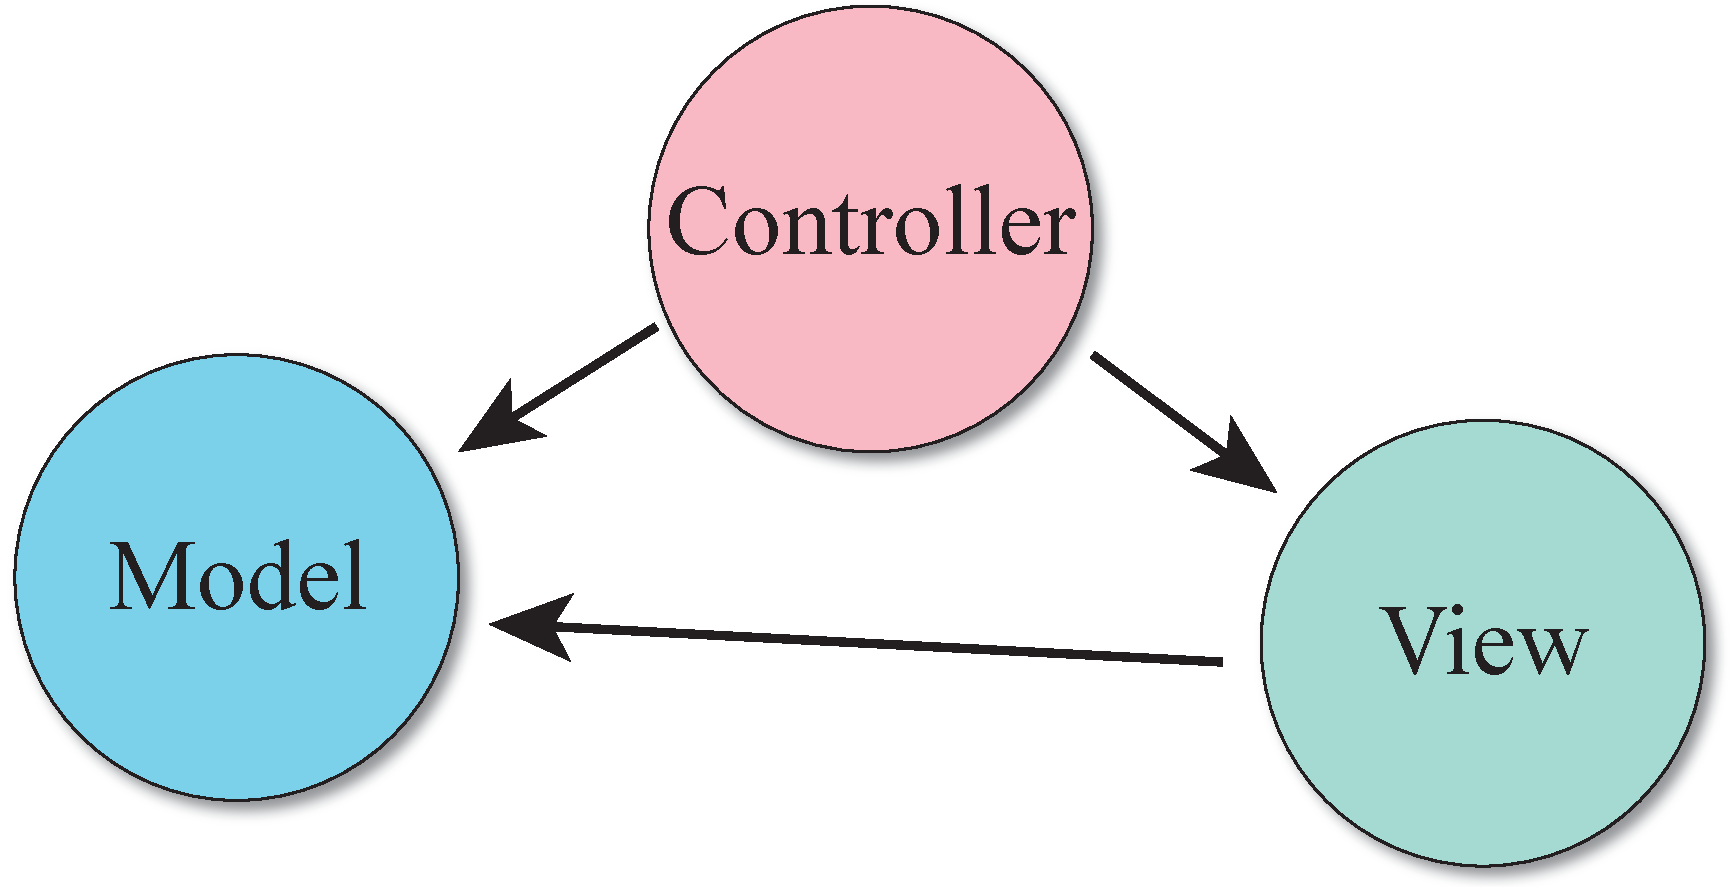
\includegraphics[width=10cm]{fig/mvc}
	\caption{Direkte Assoziationen zwischen Model, View und Controller}
\end{figure}

\paragraph{Model:}
Verantwortlich für alles, was die Daten eines bestimmten Models angeht. In der Anwendung ist dieser Bereich für Interaktionen, Gültigkeit und Auswertung verantwortlich und repräsentiert hier zum Beispiel eine Veranstaltung, ein Benutzer, Statistiken oder Koordinaten der Benutzer.

\paragraph{View:}
Generiert das Aussehen einer bestimmten Seite. Hier wird vorwiegend mit gängigen Webformaten, wie HTML, PHP und JavaScript gearbeitet. Ein View kann auf die Daten zugreifen, die ihm der Controller liefert und diese dann anschaulich darstellen. Dadurch muss sich ein View nicht darum kümmern, woher er seine Informationen zusammensuchen muss, sondern bekommt garantiert, dass diese vom Controller bereit gestellt werden. Auf diese Weise können verschiedene Views für verschiedene Geräte erstellt werden und erlauben einfach eine mobile Seite zu generieren.

\paragraph{Controller:}
Hier findet die gesamte Logik und Aufbereitung der Daten statt, die später dem Benutzer im View angezeigt werden sollen. Sämtliche Datenbankabfragen, Berechnungen oder Ähnliches werden hier durchgeführt und dem Model / View bereitgestellt. Für jedes Objekt existiert ein eigener Controller. Diese werden \emph{EventsController}, \emph{UsersController} etc. genannt.\\
In diesem Framework ist jede Funktion direkt mit den Views verknüpft, das heißt definiert man im EventsController eine Funktion namens \emph{index()}, so stellt dies eine Seite der Webanwendung dar, die mit \emph{http://localhost/Events/index} aufgerufen werden kann und den entsprechenden View in \emph{/View/Events/index.ctp} erwartet.\par

Die Vorteile bei diesem Entwurfsmuster liegen auf der Hand: Es muss nur einmal ein Objekt im Model definiert werden. Im Controller wird die komplette Logik verarbeitet und damit kann man mit entsprechenden Views für verschiedene Ansichten (z.B. eine mobile Anwendung der App) einfach auf die Daten des Controllers zugreifen. Der Code kann dadurch kompakter gehalten werden und muss nur im Controller angepasst werden, um auf allen Ansichten der Seite die Daten aktualisieren zu können.

%%%%%%%%%%%%%%%%%%%%%%%%%%%%%%%%%%%%%%%%%%%%%%%%%%%%%%%%%%%%%%%%%%%%%%%%%%%%%%%%%%%%%%%%%%%%%%%%%%%%%%%%%%%%%%%%%%%%%%%%%%%%%%

\section{Datenbanken}
Um alle Daten schnell und einfach verarbeiten zu können, ist eine Datenbank nötig. Da es sich hier um eine Webanwendung handelt, bietet sich eine SQL Datenbank an, weil diese in der Regel zum Komplettpaket eines Webservers gehört.\\
Folgende Tabellen wurden angelegt:

\paragraph{users:}
Ein Benutzer besteht aus einer eindeutigen Identifizierungsnummer (\emph{ID}), einem Benutzernamen, einem Passwort und einer zugewiesenen Rolle (z.B. Administrator, Benutzer usw.). Dazu werden von der App automatisch zwei Zeitstempel mit Erstellungs- und letztem Änderungsdatum sowie einem Boolean hinzugefügt, welcher angibt, ob der Benutzer sich im System der Webanwendung einloggen kann und damit Daten einsehen kann.

\paragraph{events:}
Jede erzeugte Veranstaltung wird hier hinein gespeichert. Verpflichtende Felder sind ein Titel und eine Beschreibung. Dazu wird von der App eine eindeutige ID zugewiesen und die Benutzer-ID des Benutzers hinzugefügt, welcher diese Veranstaltung erstellt. Dazu noch zwei Zeitstempel: Erstellungsdatum und Zeitpunkt der letzten Änderung.\par

Dies sind die beiden grundlegenden Tabellen, die für diese Anwendung nötig sind. Jedoch besteht noch keine Verknüpfung untereinander, abgesehen von der Benutzer-ID in der \emph{events}-Tabelle.

\subsection{Verknüpfung von Benutzer und Veranstaltung}
Um einer Veranstaltung beliebig viele Benutzer zuordnen zu können, wurde die Tabelle \emph{events\_users} erstellt. Diese beinhaltet nur die Fremdschlüssel ID aus den \emph{events} und \emph{users} Tabellen.

\begin{figure}[!ht]
	\centering
	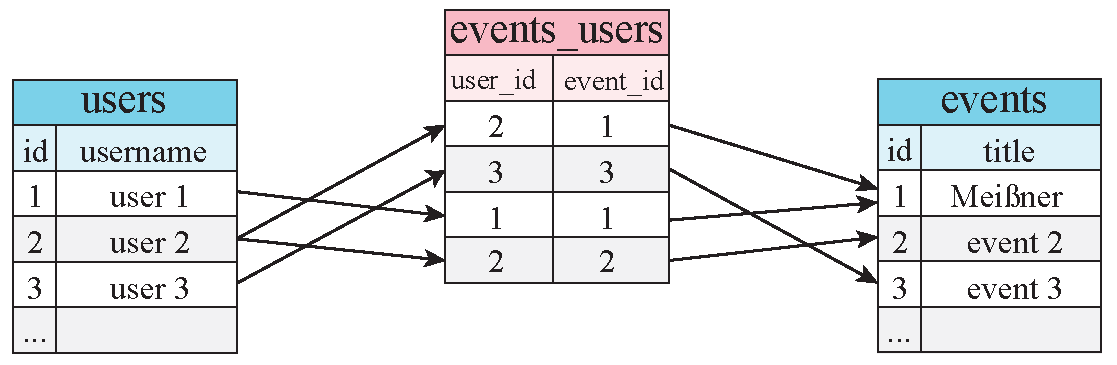
\includegraphics[width=15cm]{fig/events_users}
	\caption[Zuweisung eines Benutzers zu einer Veranstaltung]{Zuweisung eines Benutzers zu einer Veranstaltung (vereinfacht)}
\end{figure}

Diese \emph{Many-to-many}-Verknüpfung (in cakePHP auch \emph{hasAndBelongsToMany, HABTM} genannt) kann der EventsController mit einer einzigen SQL-Abfrage erfragen und erhält damit alle dem Event zugeordneten Benutzer. Diese Daten können dann in einer Variable gespeichert und dem View bereitgestellt werden.

\subsection{Veranstaltungsspezifische Eigenschaften}
Die ersten Schritte zu einer Webanwendung, die Veranstaltungen und Benutzer verwalten kann, sind nun erledigt. Bisher ist es allerdings nicht möglich in Veranstaltungen Felder zu definieren, die für eben jene Veranstaltung von Bedeutung sind. Das können im konkreten Fall Felder sein wie \glqq Art des Transportmittels\grqq{}, \glqq Wird ein Parkplatz benötigt?\grqq{}, \glqq Welcher Holzstangenbedarf besteht?\grqq{} oder Ähnliches.

\paragraph{Key-Value-Store} In einem Key-Value-Store wird die Datenbank mit den Werten (\emph{values}) über die Schlüssel (\emph{keys}) indexiert. Der Vorteil ist, dass vorher nicht bekannt sein muss, welche Werte in die Datenbank eingetragen werden sollen.\\
In der Meißner App wurde diese Methode implementiert, um eventspezifisch ein beliebiges Feld zu definieren, welches Werte als Strings annimmt. So ist gewährleistet, dass die Benutzer dieser Anwendung die größtmögliche Freiheit besitzen, was die Inhalte der Veranstaltungen angeht. Jede kann individuell angelegt und personalisiert werden, sodass sie den gewünschten Anforderungen genügt.\\
Um die häufigsten Nutzungsszenarien abzudecken, wurden Strings als Hauptformat für die Values gewählt. Diese lassen sich einfach auswerten und erhalten die einfache Bedienung der Formulare.\\
Für die automatischen Statistiken ist das Format irrelevant, da nur auf Gleichheit der Strings geprüft wird und anhand dessen die Grafiken erstellt werden. 

\paragraph{Implementierung}
Für die Implementierung sind zwei weitere Tabellen notwendig: 

\begin{enumerate} 
	\item \emph{event\_columns}: Dient als Maske, um Feldnamen und -typen zu definieren. Kann zudem innerhalb einer speziellen Veranstaltung genutzt werden, um diese Felder den zugeordneten Benutzern verfügbar zu machen.
	\item \emph{event\_properties}: Nachdem vom Controller die Feldnamen des Events abgefragt wurden, werden diese in einer Variable gespeichert und dem View übergeben. Im View wird dann ein Formular generiert, welches die Feldnamen aus \emph{event\_columns} anzeigt und die Möglichkeit gibt, Werte einzutragen. Diese Werte werden dann über den Controller in \emph{event\_properties} gespeichert.
\end{enumerate}

Mit den Tabellen steht nun die Datenstruktur zur Verfügung, die es ermöglicht verantstaltungsspezifische Eigenschaften zu erstellen und die so erzeugten Felder mit den entsprechenden Werten der Teilnehmer dieser Veranstaltung zu befüllen.

\begin{figure}[!ht]
	\centering
	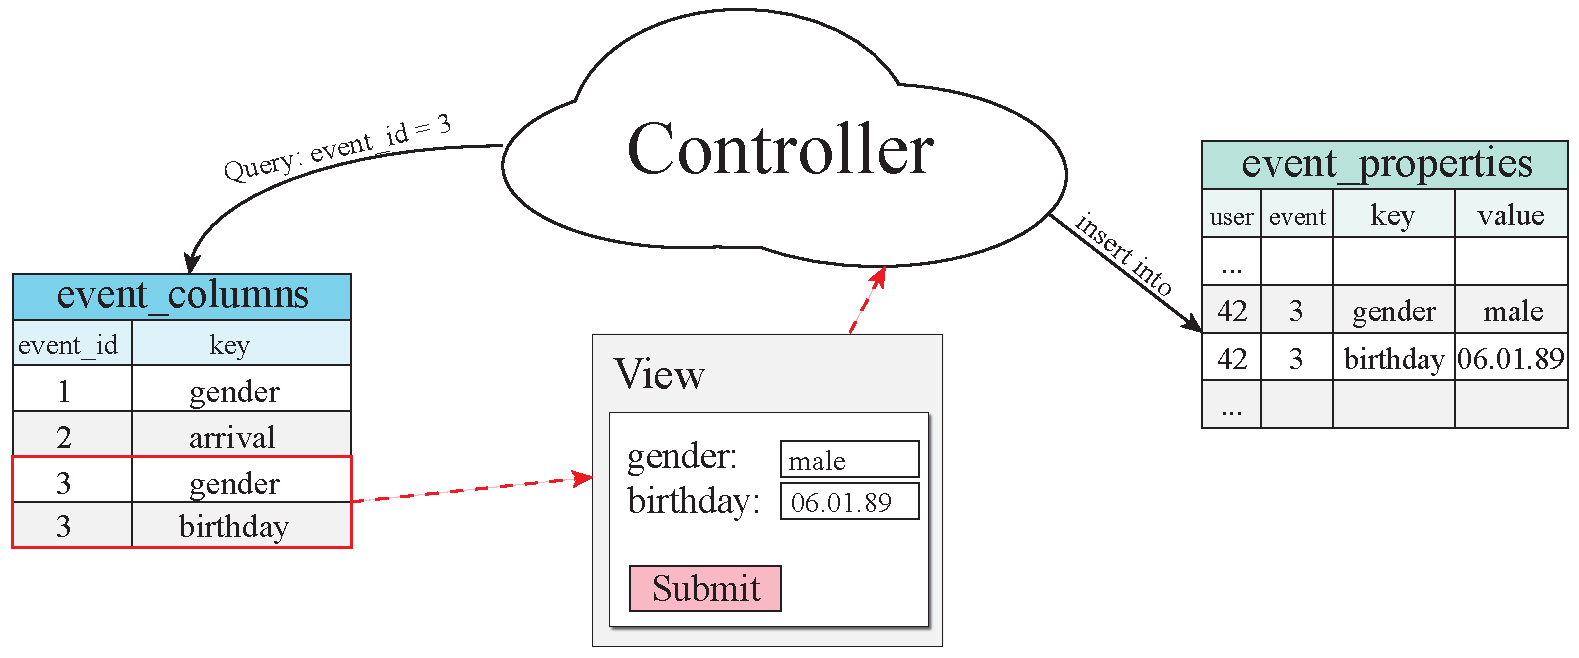
\includegraphics[width=15cm]{fig/event_properties}
	\caption[Speichern von spez. Feldern in die Datenbank]{Controller erfragt Felder aus event\_columns, stellt sie dem View zur Verfügung, speichert danach die Werte in event\_properties}
\end{figure}

Obige Abbildung zeigt kurz das Zusammenspiel von Controller und View: Datenbankzugriffe werden über den View an den Controller gerichtet und dort ausgeführt. So können Daten abgefragt oder neue Daten geschrieben werden.\par

Als einzigartige primäre Schlüssel werden \emph{user\_id} und \emph{key} gewählt, womit automatisch Duplikate ausgeschlossen werden. Somit kann immer nur genau ein Wert in einem benutzerspezifischen Feld stehen.\\
Beispiel: In der Abbildung existiert die Zeile \emph{Benutzer: 42, Event: 3, Key: gender, Value: male}. Wenn der Benutzer nun das Geschlecht in dem Formular ändert und das abschickt, dann sieht die Nachricht so aus: \emph{Benutzer: 42, Event: 3, Key: gender, Value: female}. Weil das Feld \emph{key} als Primärschlüssel definiert wurde, wird dieser Eintrag überschrieben und kein neuer Eintrag in der Datenbank angelegt.

\section{Verhinderung von Angriffen}
Gängige Angriffsmethoden, wie Cross-Site-Scripting oder SQL-Injection, werden in dieser Arbeit verhindert.

\subsection{SQL-Injection}
Bei der \emph{SQL-Injection} versucht ein Angreifer durch geschicktes Manipulieren von Eingabefeldern eines Formulars, einen String zu erzeugen, mit dem er einen ungewollten Zugang zur Datenbank erhält. Schafft er das, so kann er Datensätze aus der SQL Tabelle ausgeben lassen, verändern oder sogar komplett löschen.\par

Um diese Art der Angriffe zu verhindern, haben die Entwickler von cakePHP einige Sicherheitsvorkehrungen implementiert. Zusätzlich gibt es das Modul \emph{Sanitize}, welches die Eingabestrings des Benutzers überprüft und alle Sonderzeichen, wie Hochkommata und Semikolons, aus dem String entfernt. Damit lässt sich keine zusätzliche Anweisung in den SQL-Query mit einbauen und die Anwendung ist somit weitgehend vor diesen Angriffen geschützt.

\subsection{Cross-Site-Scripting XSS}
Mit \emph{XSS} beschreibt man eine Angriffsmethode, die Webseitenübergreifend Schadcode über normale Hyperlinks ausführt. Dabei können bei Clients, die JavaScript unterstützen, Cookies an den Angreifer übertragen werden.\par

Auch hier übernimmt cakePHP das Abwehren dieser Angriffe. Damit diese Mechanismen auch greifen, werden in dieser Webanwendung die von den Entwicklern vorgeschlagenen Paradigmen beachtet.

%%%%%%%%%%%%%%%%%%%%%%%%%%%%%%%%%%%%%%%%%%%%%%%%%%%%%%%%%%%%%%%%%%%%%%%%%%%%%%%%%%%%%%%%%%%%%%%%%%%%%%%%%%%%%%%%%%%%%%%%%%%%%%

\section{Views entwickeln}
Nun wurde mit modernen Webtechnologien und möglichst geringem Aufwand direkt eine mobile Seite der Anwendung erstellt, welche für Smartphone und Tablets optimiert ist. Schließlich soll und muss diese Web-App auch auf dem Gelände mobil genutzt werden können.\par

Dabei gibt es mehrere Ansätze, wobei in dieser Arbeit das sogenannte \emph{Responsive Webdesign} (deutsch: bedarfsgesteuertes Webdesign) für die mobile Version der Anwendung benutzt wird.

\subsection{Responsive Webdesign mit jQuery Mobile}
Hauptaugenmerk wird hier auf die Auflösung des Endgeräts gelegt: Handelt es sich hierbei um ein günstiges Smartphone mit schlechtem Display, um ein Google Nexus 10 mit 2560x1600 Pixeln oder um einen SmartTV mit FullHD?\\
Diese Frage ist entscheidend, denn sie bestimmt wie viele und wie groß bestimmte Objekte im Sichtbereich des Geräts sein können, sodass der Benutzer nicht von der schlechten Bedienung genervt ist, sondern weiterhin die Informationen aus der App holen möchte. Beim Responsive Webdesign werden über \emph{Media Queries} (Abfrage der Eigenschaften des Geräts, Beispiel: Auflösung, Orientierung des Endgeräts usw.) Informationen des Endgeräts eingeholt und darauf abgestimmte Stylesheets geladen.\par

Um aber eine Webanwendung zu entwickeln, die aussieht und sich \glqq anfühlt\grqq{} wie eine echte App wurde in dieser Arbeit das Framework \emph{jQuery Mobile} verwendet, welches auch auf Responsive Webdesign setzt und dabei viele Steuerelemente zur Verfügung stellt, die dem Benutzer schon von nativen Apps her bekannt sind, wie typische Slider, Buttons, Dropdown-Menüs und vielem mehr.\par

\paragraph{Mobile View}
Damit jQuery Mobile aus normalen Verlinken touchoptimierte Bedienelemente erzeugt, konnte nahezu der komplette Code von der Desktop-Version genommen werden. Lediglich kleine Ergänzungen um das \emph{data-role} Attribut sind notwendig, damit jQuery Mobile diese anpassen kann, das bedeutet ein normaler Hyperlink wird um \emph{data-role="button"} erweitert.
\\
\begin{lstlisting}[captionpos=b, caption=Eine kleine Ergänzung erzeugt aus einem Link einen touchfreundlichen Button]
<a href="#">normal link</a>
<a href="#" data-role="button">touchoptimized link</a>
\end{lstlisting}

Auf ähnliche Art und Weise können auch viele andere Elemente umgewandelt werden, damit diese für Smartphones optimiert sind. Oft erfolgt dies automatisch, da jQuery Mobile Bedienelemente erkennt und diese dann sofort anpasst.
